\chapter{Aids to Selection --- Pedigree Estimates}
\label{cha:Lush_Chapter_14}
\index{Pedigrees as aids to selection|(}

\begin{quote}
``The bull gives no milk, of course, yet will not a bull descended from several generations
of high-producing dams produce, when mated with a highly productive cow,
calves which possess this characteristic to a still higher degree?'' --- Bergen, in 1780.
\end{quote}

The decision of whether to reject or keep an animal for breeding
may be modified by what its relatives are or do. Wherever that is done,
the intensity of individual selection is reduced. The average individual
merit of those selected must be lowered every time an animal which
would be rejected on account of its own individuality is kept for breeding
because it has unusually excellent relatives, or every time an individually
excellent animal is rejected because its relatives are of low
merit.

By paying a reasonable amount of attention to the relatives it may
be possible to increase the genetic accuracy of the selections more than
enough to offset the decrease in the intensity of selection for individual
merit. There is real danger of doing damage by paying too much attention
to the relatives, since they are not a perfect guide to the individual's
breeding value either. The proper balance between paying too
much and paying too little attention to the merits of the relatives shifts
from case to case according to how well the merits of the relatives are
known, how closely they are related to this animal, how well the individual
merit of this animal is known, and how highly hereditary the
characteristics are. An understanding of the principles and practical
difficulties involved will help in using the approximate rules which in
actual practice must guide us in estimating an individual's breeding
value from what we know about the merit of its relatives.

From the genetic principles involved, relatives of an individual may
all be grouped in two classes: those which are related to it through its
parents and those which are its descendants. The former group is considered
here collectively under the general term of ``pedigree,'' which is
the subject of this chapter, while the latter group will be considered in
the next chapter under the term of ``progeny test.''\index{Progeny test}

Attention to pedigree can make selection more effective only
because individual selections are not perfectly accurate. We never know
exactly what genes an individual has. Our knowledge of that is especially
scanty when the animal is still immature, as many are when first
selections must be made. If we estimate its inheritance from its own
appearance or performance, we will make some mistakes on account of
the effects of environment, dominance, and complex interactions of
genes. If we estimate its inheritance by paying attention to the individuality
and performance of its relatives, we may avoid some of those
mistakes; but we run the risk of introducing other mistakes, because
those relatives will not have exactly the same genes as this animal does.
Moreover, our estimate of the genes in those relatives is itself subject to
error from our being confused by the effects of dominance, environment,
and complex gene interactions on those relatives.

\section*{GENERAL PRINCIPLES WHICH LIMIT THE USEFULNESS OF PEDIGREES}
\index{Sampling nature of inheritance|(}

The biological basis for the usefulness of pedigrees lies in the fact
that an individual gets half of its inheritance from its sire and half from
its dam. If we knew what inheritance these parents had, we could estimate
what inheritance this individual probably received from them.
Because the parents were heterozygous for some of their genes, such
estimates cannot be perfectly accurate. Chance at Mendelian segregation
plays a part in determining what the parents transmit to any one
offspring. An additional limitation on the use of pedigrees is that we
will rarely know exactly what genes the parents did have, although we
will often know more about their inheritance than about the inheritance
of each of the offspring, because the parents have had a longer
time in which to demonstrate their characteristics or performance. Also,
because some of the ancestors will have had other offspring, they will be
to some extent progeny-tested, whereas most individual selections must
be made before any progeny are available.

Even if we knew exactly what genes each parent had --- and no
amount of pedigree study could tell us that much --- the sampling nature
of inheritance limits the average likeness between the inheritance of an
individual and the inheritance of either parent in a random breeding
population to a correlation of $+$ .50. On the same basis the correlation
between an individual and the average of its two parents is $+$ .71. If
much inbreeding, or mating of like to like where ideals are diverse, is
being practiced, these correlations will be larger; but in any actual
population they will be far from perfect. If we are trying to predict the
average merit of many offspring, the effects of chance at segregation will
tend to cancel each other. The correlation between the inheritance of
one parent and the average kind of inheritance of $n$ of its offspring
approaches $+$ 1.00 according to the formula \(\sqrt{\dfrac{n}{n + 3}}\)
if the other parents of those offspring are a random sample of the breed. The correlation
between the average inheritance of both parents and the average
inheritance of $n$ of their offspring approaches $+$ 1.00 according to the
formula \(\sqrt{\dfrac{n}{n + 1}}\).\footnote{\textit{See also} page 260.}
These correlations are between genotypes and not between the directly
observable characteristics of the animals, but the formulas explain what
seems at first to be a contradiction between the facts that pedigrees cannot
be highly accurate for estimating what an individual animal will be and yet
can be very accurate in predicting the average qualities of a large number
of offspring from one pair of parents.
\index{Sampling nature of inheritance|)}

\index{Ancestors, importance of various ones|(}
If we knew exactly what genes the sire and dam each had, nothing
would be gained by considering more distant ancestors or collateral
relatives. Figure~\ref{fig:Lush_Figure_25} shows a Mendelian example
of that with respect to one pair of genes.

\begin{figure}
	\centering
    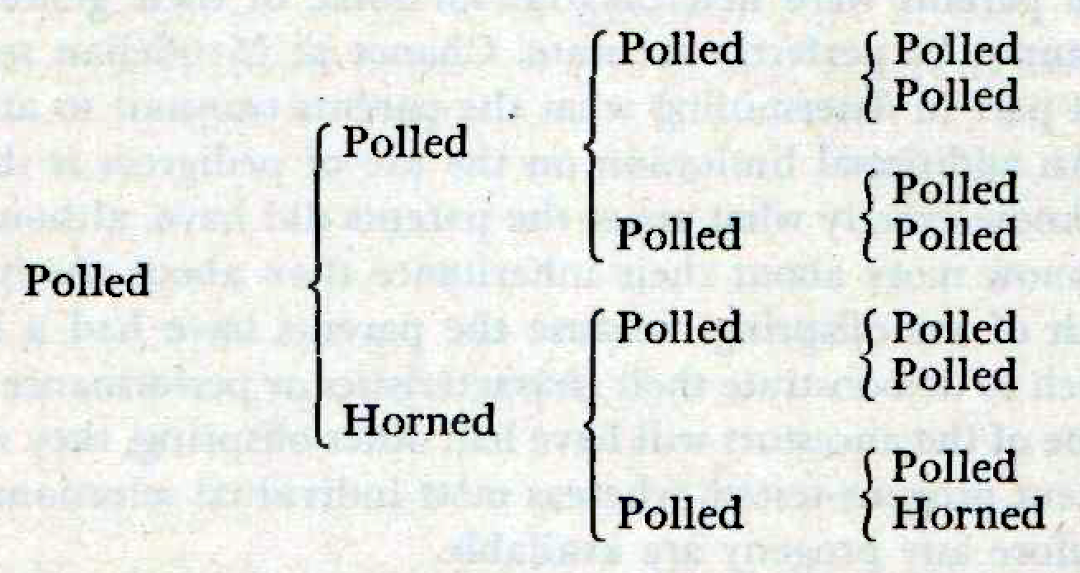
\includegraphics[width=\textwidth]{Figure_25.png}
    \caption{A pedigree of a Polled Hereford, illustrating the general principle that
			 study of remote ancestors tells nothing more about an animal's inheritance when the
			 genotype of an intervening ancestor is known with certainty.}
    \label{fig:Lush_Figure_25}
\end{figure}

Insofar as we are correct in thinking that horned cattle are \textit{pp} and
polled cattle are either \textit{PP} or \textit{Pp}, it is certain that the dam
in Figure~\ref{fig:Lush_Figure_25}
was \textit{pp} and that this offspring of hers is \textit{Pp}. No amount of study of her
ancestors would add anything to our knowledge of that. That brings us
to the question of how much attention to pay to each ancestor in the
general case where we know something about the individual merit of
most ancestors but are not entirely sure of the genotype of any of them.
The answer to that question depends on five different circumstances:
First, how closely the ancestor is related to the subject of the pedigree;
second, how completely the merit of each ancestor is known; third, how
well the merit of intervening ancestors is known; fourth, how highly
hereditary the characteristic is; fifth, how much environmental correlation
there is between ancestor and subject and between different
ancestors.

The general fact that an animal gets half of its inheritance from
each parent would naturally lead to one form of what is generally called\index{Galton's ``Law''}
``Galton's law'' --- of which more is said in chapter 20 --- namely: In estimating
an individual from knowledge about one of its parents, it
should be estimated as equal to one-half of that parent plus one-half of
the breed average; if it is being estimated from a grandparent, it should
be estimated at one-fourth of that grandparent plus three-fourths of the
breed average; with a great grandparent, it should be one-eighth of that
great grandparent plus seven-eighths of the breed average, etc. The
importance of the ancestor in such a prediction equation is halved with
each additional generation which intervenes between the individual
and its ancestor. This ``law'' in general is sound in a random breeding
population, provided only one ancestor is being considered and provided
some conservatism is practiced by basing a smaller share of the
estimate on the ancestor and a correspondingly larger share on the
breed average wherever the characteristic is not highly hereditary or
there is uncertainty that the information about the ancestor really is a
true picture of its inheritance. Two ancestors cannot both be used in a
single prediction of this kind if one of them is an ancestor of the other.
We could combine information about the sire and the maternal grandsire,
estimating the animal at one-half of the sire plus one-fourth of the
maternal grandsire plus one-fourth of the breed average, with still more
emphasis on the breed average as we are less sure that what we know
about the sire and grandsire is really typical of their breeding value.
But we could not combine information about the sire and the paternal
grandsire in the same way because, to a considerable extent, the things
which could be estimated from knowledge of the grandsire are the same
things which could be estimated better from knowledge of the sire himself.
The use of both in a single prediction would be using some of the
information a second time.

Czekanowski\footnote{Zeit. f. Ind. Abst. u. Vererbungslehre 64:154--68. 1933.}
has explored the question of the comparative importance
of sire, grandsire, and great grandsire in the special case when (1)
all three are in the same line of descent, (2) no other ancestors are considered
(3) exposure of relatives to the same kind of environment has
contributed nothing to the correlation between them, and (4) the merits
of all three ancestors are equally well known. His figures for the
amount of attention (the net regression coefficient) to be given each of
these three ancestors for several values of the correlation between parent
and offspring are as follows:

\begin{table}[htbp]
	\centering
	\begin{tabular}{l|c|c|c|c|c|c|c}
		\hline
		\hline
		 				& \multicolumn{7}{c}{Correlation Between Parent and Offspring} \\
		 				\cline{2-8}
		 				& .10 &	.20 &	.25	& .33	& .40	& .44	& .50 \\
		\hline
		Sire			& .095	& .186	& .232	& .312	& .381	& .431	& .500 \\
		Grandsire		& .039	& .059	& .062	& .059	& .046	& .030	& .000 \\
		Great grandsire	& .016	& .020	& .018	& .012	& .006	& .002	& .000 \\
		\hline
	\end{tabular}
\end{table}

\noindent
The figures show how little is to be gained by considering the remote
ancestors when the merit of the intervening ones is equally well known.
For highly hereditary characteristics the sire's own appearance or performance
is almost a perfect guide to the net worth of his inheritance.
For slightly hereditary characteristics, relatively more attention should
be paid to the remote ancestors, but in that case the predictive value of
pedigree is low anyhow, no matter how used. It is doubtful whether
Czekanowski's figures have any practical usefulness beyond demonstrating
these genera l principles. In actual practice some ancestors will
be much better known than others. For example, if the sire in Czekanowski's
problem were still too young for his mature characteristics to
be unmistakable or if the grandsire were thoroughly progeny-tested\index{Progeny test},
less attention should be given to the sire and more to the grandsire than
these figures indicate.

\index{Collateral relatives}
Collateral relatives in the pedigree are a progeny test which furnishes
evidence about the genotypes of their parents or grandparents.
Although a grandparent is generally as good an indicator of an individual's
inheritance as a half brother or sister, an individual can have
only four grandparents but may have a much larger number of half
brothers and sisters. In case it does, an estimate of its inheritance based
on the appearance and performance of its half brothers and sisters may
be much more accurate than an estimate based on its grandparents. The
evidence furnished by collateral relatives should be used in the pedigree
according to what it shows about the kind of inheritance which
the mutual ancestor had and according to the completeness of the evidence.
For example, in a dairy pedigree where the production of a
large number of paternal half sisters is known, the sire may be considered
reasonably well proved, and there is little to be gained by studying
his ancestors. If the dam in the same pedigree is still a young cow in her
first lactation, considerable information could be gained by considering
the maternal grandparents, although consideration of the paternal
grandparents would be of little use.
\index{Ancestors, importance of various ones|)}

The chief danger in pedigree selection is that it will do more harm
by lowering the intensity of individual selection than it does good by
making the selection more accurate. Pedigree is not often as accurate a
basis for estimating breeding value as individuality is,\footnote{In a random
breeding population in the limiting case most favorable to confidence
in the pedigree --- the case where the genotypes of sire and dam are perfectly
known --- the correlation between an animal's breeding value and its own individual
appearance or performance is \(\sqrt{2a}\) times as large as the correlation between its breeding
value and the average genotype of its parents, where $a$ is the additive genetic
fraction of the variance in individual appearance or performance. This relation indicates
the basis for the general principle that pedigree can become more dependable
than individuality for characteristics which are slightly hereditary (i.e., where $a$ is
less than \nicefrac{1}{2}), provided the parents are so thoroughly known that there is little
doubt about their genotypes.} although it will
occasionally be so in a hitherto unselected population, especially if the
individuals being selected are still too young to have had much chance
to prove their characteristics at the time the selection must be made.
Pedigree selection is rarely as useful in animal breeding as it can be at
times in plant breeding, because there is almost nothing in animal
breeding to correspond to the distinct and uniform lines or families
which exist in those plant species, such as wheat and cotton, where self-fertilization
or some other intensive form of inbreeding is the rule. In
plants in which self-fertilization is possible, an individual may have
only one parent, only one grandparent, one great grandparent, etc., and
each of these may be more thoroughly progeny-tested than is possible
where reproduction must be bi-parental.

\section*{PRACTICAL LIMITATIONS ON THE USEFULNESS OF COMMERCIAL PEDIGREES}

Often pedigrees contain little information except the names and
numbers of the ancestors. To use them at all, you must find from other
sources how excellent or poor those ancestors were. That is less true of
dairy and poultry pedigrees than of others and is being improved in the
pedigrees of most kinds of livestock; but, as printed today, many pedigrees
are only a meaningless genealogical jumble of names and numbers
to one who does not know from other sources how meritorious
those ancestors were. This limitation does not matter much to the man
who is thoroughly familiar with his breed. Perhaps all purebred breeders
should aim at that goal, but an enormous number of potential customers
and even many breeders simply have not time nor opportunity
to keep familiar with the merits and deficiencies of the prominent
breeding animals of their breed. Pedigrees would be more useful to
these men if more information were included about the merits of the
ancestors, even if that meant only printing the pedigree as far the
parents and grandparents. In justice to those who print the pedigrees,
it should be emphasized that in most cases there is no information to
print because no systematic plan of measuring and recording the merit
of individual animals has ever been in operation.

This is no new idea. As long ago as 1832 the following was written
in \textit{The Thoroughbred Horse in Prussia}: ``If they do not contain production
tests, such herdbooks will be useless and without interest, since
they would contain only names of which no one knows anything and
which mean nothing.''

Such information as is given in the pedigrees is usually selected to
show the animal in the most favorable light possible. Actual falsehoods
in printed pedigrees are rare because of the heavy penalties in loss of
business which are exacted of a breeder who is suspected of dishonesty;
but plenty of \index{``Filler'' in pedigrees|(}``filler'' is still used,
although general practice in this
respect is improving. An example of ``filler'' is shown in Figure~\ref{fig:Lush_Figure_26}. The
information printed under an ancestor's name applies in many cases to
half sisters of its parents or grandparents or even to more remote relatives.
The following statement was found listed under the paternal
grandsire in a pedigree of a bull used in a large dairy herd in Iowa in
1937. ``His dam is a granddaughter of that noted transmitter, Sir
$\cdots\cdots$, sire of $\cdots\cdots$'' The actual records
mentioned here were made by cows separated by six Mendelian segregations
from the bull in whose pedigree they appeared, and related to
him less than 2 per cent. By contrast Figure~\ref{fig:Lush_Figure_27} shows a pedigree in
which each bit of information is listed under the ancestor which it most
directly concerns.
\nowidow

Generally the ancestors were selected individuals from among their
contemporaries. That is especially likely to have been true of the males
and hence of their ancestors. Some regression to the breed average is to
be expected for that reason, even if the pedigree information is supplied
by an utterly impartial and accurate agency. The intensity of the
selection practiced in choosing those ancestors is not usually known.

In most pedigrees little information is given about collateral relatives.
That is beginning to be remedied in dairy cattle and poultry
pedigrees by the inclusion of progeny tests wherever those are available.
Occasionally in the pedigrees of meat animals one finds comments
on the winnings or performance of brothers or other collateral relatives.
Information about \index{Collateral relatives}collateral relatives may be much more highly
selected than information concerning ancestors, since there can be no
choosing of ancestors to be mentioned but only selection of data
concerning them; whereas among the \index{Collateral relatives}collateral relatives there may be
choice of which individuals shall be mentioned and also selection of
the best records of those individuals. One often finds in dairy pedigrees
such comments as ``20 A.R. daughters, two with over 1,000 pounds of
fat.'' Since the records of 18 of the 20 are omitted and the number of
daughters not tested is not stated, such a statement tells little more than
that this sire was used extensively and was regarded highly enough that
20 of his daughters were tested officially.

\begin{figure}
	\centering
    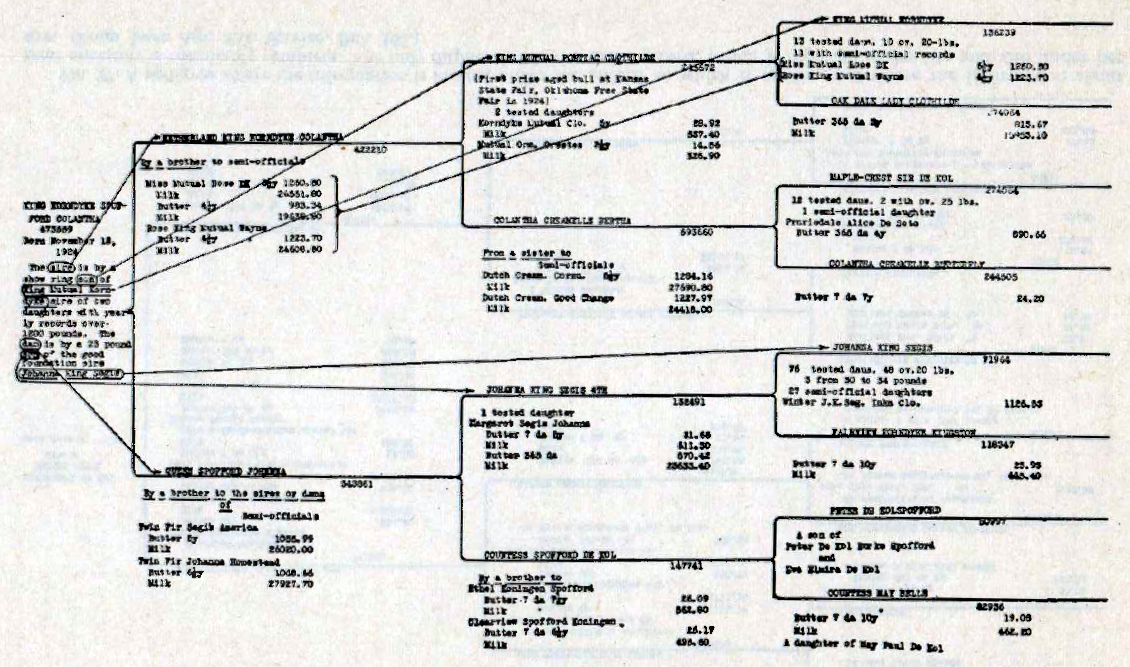
\includegraphics[width=\textwidth]{Figure_26.png}
    \caption{A pedigree showing a moderate amount of ``filler.'' Favorable
    		 items are repeated several times and are placed under animals
    		 rather distantly related to those on whose inheritance the
    		 items throw most light. (From Iowa Agr. Ext. Service, Bul. 162.)}
    \label{fig:Lush_Figure_26}
\end{figure}

\index{``Filler'' in pedigrees|)}

\begin{figure}
	\centering
    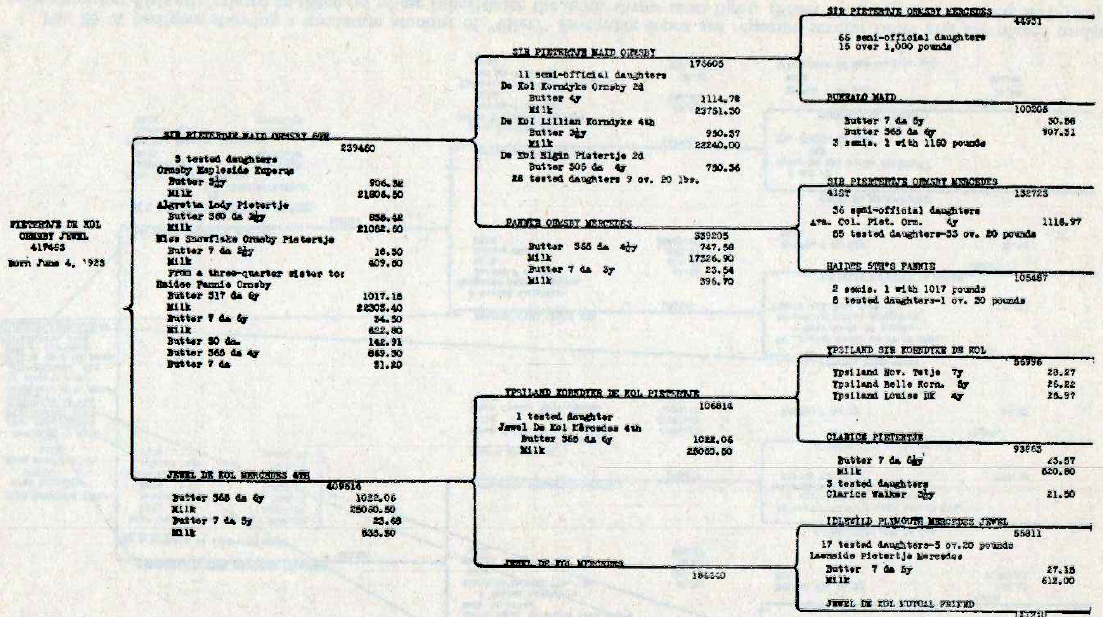
\includegraphics[width=\textwidth]{Figure_27.png}
    \caption{A pedigree showing a moderate amount of ``filler.'' Favorable
    		 items are repeated several times and are placed under animals
    		 rather distantly related to those on whose inheritance the
    		 items throw most light. (From Iowa Agr. Ext. Service, Bul. 162.)}
    \label{fig:Lush_Figure_27}
\end{figure}

Usually no average pedigree of the breed is available for comparison
with the one being considered. That lack would not bother the man
who has studied enough pedigrees of his chosen breed to get a fairly
definite idea of what a typical pedigree is, but many people simply cannot
spare the time for such study or <lo not have access to enough pedigrees
to learn what is typical for the breed.
\noclub

In a sense individual select ion is pedigree selection for the next
generation. When the parents have been selected for individuality, the
offspring which would have had the worst pedigrees are not permitted
to be born! Much of the use which might be made of pedigree selection
in a hitherto unselected population is simply not available to the breeder
who is pursuing the same goal which was pursued by those who bred
and selected the parents of his animals. This sets further limits to the
usefulness of pedigree selection under ordinary practical circumstances.
There are some exceptions to this general situation. One is the fact that
fewer males than females are needed for breeding. After the males are
born there can be much pedigree selection among them, although there
cannot be much among females. This is what a cattle breeder does when
he decides he will save a calf from a certain cow if it is a heifer but not if
it is a bull. When a breeder's ideals differ distinctly from those of many
of his fellows and he lays much importance on things which they consider
unimportant and vice versa, the pedigrees of their animals offer
him considerable opportunity for selection if he purchases from them.
Also, when the ideal of a breed changes, there is momentarily a reappraisal
of the merits of the ancestors. While that is happening there is
opportunity for pedigree selection on the new basis for a generation or
two. Selection among the parents does not reduce the variability among
their offspring nearly as much as it does the variability among the parents
themselves. Hence in a population which has already been under
selection for a generation or two there is much more opportunity for
selecting the offspring on their individuality than on their pedigrees.

\section*{ERRORS WHICH MAY BE CORRECTED BY PEDIGREE SELECTION}

Pedigree selection helps to overcome deception by environment
because it does not often happen that the ancestors were all kept under
the same environment.

Pedigree study would be of some help in overcoming deception by
\index{Dominance}dominance if full information about the collateral
relatives were presented,
but that is rarely done. If the recessive is rare and only the direct
ancestors are given, pedigree is almost no help in this respect. For example,
pedigrees do not help in eliminating red in the black breeds of
cattle, since all ancestors are black and the existence of red sibs or aunts
or uncles or other collateral relatives is not mentioned. The parents of
red calves and something more than half of the sibs of red calves are
heterozygotes. Culling them because of their relationship to the red animal
would make the genes for red scarcer than can be done by culling
the red alone, but present pedigrees do not give the information which
would permit that. Nor is it likely that breeders would report such
information if it were to be used to reflect unfavorably upon animals
they have for sale. Pedigrees help a little in overcoming deceptions by
dominance in such cases as the polled Herefords where the distinction
between horned and polled is shown in the pedigree.\footnote{The
probability that a polled calf from polled parents is homozygous for the
gene for polledness is equal to \(\dfrac{1 + s + d + sd}{3 + s + d - sd}\)
where $s$ is the probability that the sire is \index{Homozygosis}homozygous and $d$ is the
probability that the dam is homozygous. Probability is expressed on a scale
ranging from zero for absolute impossibility to 1.0 for absolute
certainty.}

Pedigree studies may help considerably in overcoming the deceiving
effects of \index{Epistatic effects}complex gene interaction. An unusually good animal from
poor or mediocre stock on both sides always suggests that this animal is
the result of a lucky combination of several genes all of which are necessary
in order to permit each to manifest its desirable effects. The occurrence
of such an animal is often called ``nicking.'' In that case the
animal would almost certainly be heterozygous for many of the genes
whose cooperation is required. There would be small chance of its
transmitting enough of those genes in each gamete to cause this excellence
to reappear in many of its offspring. Likewise, a poor individual
with excellent ancestors and relatives on both sides will be suspected of
lacking just a few genes which are necessary for the successful operation
of the other genes for the excellent qualities of his family. It will be suspected
that he has many good genes which do not manifest their presence
in him. If he were used for breeding, many of his mates would
transmit to their offspring the necessary genes he lacks. He may be preferred
to a better individual from a poorer family, although, of course,
he would be discarded if there were enough good individuals in his own
family.

\section*{RULES FOB THE USE OF PEDIGREES IN SELECTION}

In evaluating a pedigree one should estimate what kind of inheritance
the sire and the dam had and then average those two estimates.
Wherever there is uncertainty about an individual's inheritance, conservatism
requires that it should be estimated closer to the average of
its breed or herd than the evidence about it, if accepted at face value,
indicates it to be. Thus, if there is much evidence about the sire but
only a little about the dam, the estimate should give much weight to the
sire but most of the weight which would have gone to the dam should
be placed on the breed or herd average\index{Regression}. The estimate of the sire's inheritance,
or of the dam's inheritance, is made similarly by averaging the
inheritance of its sire or dam and then modifying that average by what
its own individual merit seems to be, using the general principle that
the individual's own merit should receive more weight than its pedigree
under most circumstances. For characteristics which are but slightly
hereditary or in cases where the ancestors' merits are much better
known than the individual's merit --- as, for example, where the ancestors
are well progeny-tested or have long lifetime records while the individual
is still immature --- it may be correct to attach more weight to
pedigree than to individual merit.

The more certainly an ancestor's merit is known, the less weight
should be placed on its ancestors. This is difficult to place on a quantitative
basis, but Czekanowski's table will give a rough idea of about
what that relation should be when two ancestors in the same line are
equally well known. If the breeding value of the nearer ancestor is
known with much more certainty than that of the more remote ancestor,
there is scarcely any use to pay attention to the more remote
ancestor.

If there is reason to think that much sex-linkage\index{Sex linkage} is involved in a
particular case, the proper procedure is to give the sire more weight in
estimating the inheritance of female offspring and to give the dam more
weight in estimating the inheritance of male offspring. (See page \pageref{page255}
for reasons.) The principle of conservatism in cases where the merit of
the two parents is not equally known can also give rise to unequal
weighting. Thus, in dairy pedigrees where the sire is too young to be
progeny-tested but the dam's production is known, much weight can be
placed on the dam, but only a little on the sire on account of the uncertainty
about the sire's side of the pedigree. In another dairy pedigree
where the sire is well progeny-tested but the dam is a young heifer in
her first lactation, the situation may be reversed, with more weight
being put on the sire's side of the pedigree, only a little on the dam,
some on her pedigree, and much on the breed average for conservatism
in her case.
\noclub[3]

Because the ancestors are in most cases selected animals and
because the information about them is selected to show them in a favorable
light, allowance should be made for regression toward the breed
average. There seems to be no quantitative rule for doing that except
the general one that the more extreme the selection is believed to have
been among the parents or in the information presented concerning
them, the more allowance should be made for regression.
\nowidow

\section*{SUMMARY}

The accuracy of pedigree selection is limited because of the sampling
nature of inheritance wherever genes are heterozygous. This
makes it impossible to be exactly sure of what an individual offspring
will be, even if one were in the extreme position of knowing exactly
what inheritance its sire and dam had.

The accuracy of pedigree selection is further limited in practice
because one is never entirely sure of the inheritance the parents had,
since that, too, must be estimated from their own appearance or performance
or from that of various of their relatives.

A limited amount of attention to pedigree will make the selections
more accurate, but it necessarily cuts down on the intensity of the individual
selection which can be practiced. Too much attention to pedigree
may do more harm by decreasing the intensity of individual
selection than it will do good by increasing accuracy, since pedigree
selection is not perfectly accurate either.

The use of pedigrees is based on the principles: that inheritance is
approximately equal from sire and from dam, and that, wherever one's
knowledge of the inheritance of the relatives is uncertain, one should be
conservative and estimate that the individual is somewhat nearer to the
breed average than the performance of its relatives.

Rarely should the pedigree receive as much weight as the animal's
own appearance or performance, although that can happen for slightly
hereditary characteristics if the merit of parents and grandparents is
much better known than the individual's own merit, either because
those ancestors are well progeny-tested or because the individual is still
too young to show its merits as unmistakably as its parents and grandparents
do.

Collateral relatives constitute progeny tests of some ancestor. They
therefore make the estimate of its inheritance more certain. If an animal
is well progeny-tested, little will be gained by studying the ancestors
back of it in the pedigree.

The proper amount of attention to pay to different relatives
depends on the closeness of their relationship to the subject of the pedigree,
upon how many of them there are, upon how completely the merit
of each other relative is known, and upon how highly hereditary the
characteristic is.
\nowidow

Because the ancestors are usually selected individuals, some regression
toward the breed average is to be expected . Moreover, the information
about the ancestors is usually selected to make them appear in the
most favorable light. For that reason more regression is to be expected.
Serious defects in the practical use of pedigrees include the fact that
the merit of collateral relatives such as sibs, uncles, cousins, etc ., is rarely
mentioned. If it is mentioned, it usually concerns only certain individuals
selected to make the pedigree more attractive and, moreover, is
selected information about those.

In most commercial pedigrees, other than those for dairy cattle and
poultry, little information of any kind is included except the names
and identifying numbers of the animal. Such a pedigree is useful only
to the extent that one knows or can find from some other source how
meritorious or mediocre those ancestors were.

In a breed which has been selected steadily toward the same goal for
two or more generations, there often is only a little room to practice
pedigree selection because the worst individuals among those which
might have become ancestors were eliminated by individual selection.
Therefore, the individuals which might have had the worst pedigrees, if
there had been no selection, simply do not get born.

The general conclusion regarding pedigree selection is that it should
usually be a minor accessory to individual selection, being permitted to
sway the balance in making decisions which are fairly close on individual
merit. It is most needed for characteristics which are not very
hereditary, for characteristics which only one sex can manifest, and
in selections which must be made while the animals are yet too young
to show clearly in their own appearance or performance what their
individual merit is.

The kind of errors in individual selection which are most likely to
be remedied by pedigree selection are those arising from the immaturity
of the individual and from mistaking differences caused by environment
and epistatic interactions for differences in breeding value. It
helps remedy errors caused by dominance when fairly full information
about collateral relatives is included, but is not of much help in this
respect when only the ancestors are described.

\section*{REFERENCES}

\begin{hangparas}{0.5in}{1}%
Marshall, F. R. 1911. Breeding farm animals. pp. 93--101.

Wriedt, Christian. 1930. Heredity in livestock. (Especially the chapter on ``Valuation
of Pedigree,'' pp . 168--72. Also pp. 6--10.) New York: The Macmillan
Company.
\end{hangparas}
\index{Pedigrees as aids to selection|)}